\documentclass[border=10pt, sans]{standalone}

\usepackage{tikz}
\usetikzlibrary{intersections}
\usetikzlibrary{calc,patterns,angles,quotes}
\usetikzlibrary{arrows}
\usetikzlibrary{shapes.arrows}
\usetikzlibrary{plotmarks}

\usepackage{tkz-euclide}
\usepackage{tikz-dimline}
\usepackage{fontawesome}

\definecolor{blueish}{HTML}{347dbe}

\tikzset{every picture/.style={/utils/exec={\bfseries\sffamily}}}
\begin{document}
  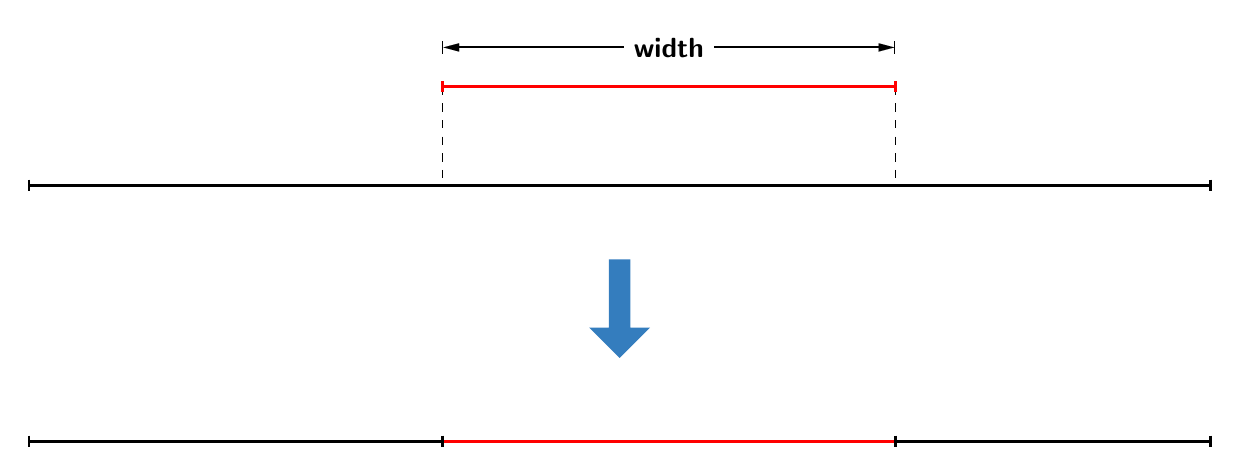
\begin{tikzpicture}[scale=1]
  	\coordinate (a) at (0,0.75);
  	\coordinate (b) at (15,0.75);
	\coordinate (d1) at (5.25,0.75);
	\coordinate (d2) at (11,0.75);
	\coordinate (p1) at (5.25,2);
	\coordinate (p2) at (11,2);

   	\draw[line width=1](a) -- (b);
   	\draw[line width=1, red](p1) -- (p2);
   	
	\dimline[
		line style = {line width=0.75},
		extension start length=0,
		extension end length=0,
	] 
	{(5.25, 2.5)}{(11, 2.5)}{width};
	
   	\draw[line width=0.5, dashed](p1) -- (d1);
	\draw[line width=0.5, dashed](p2) -- (d2);
	\draw[line width=1, red]plot[mark=|] coordinates{(5.25,2)}{};
	\draw[line width=1, red]plot[mark=|] coordinates{(11,2)}{};
	\draw[line width=1]plot[mark=|] coordinates{(0,0.75)}{};
	\draw[line width=1]plot[mark=|] coordinates{(15,0.75)}{};
	
	\node at (7.5,-0.75) [
	fill=blueish,
	single arrow,
	minimum height=1.25cm,
	rotate=-90
	] {};

  	\coordinate (d) at (0,-2.5);
	\coordinate (f) at (15,-2.5);
	\coordinate (dd1) at (5.25,-2.5);
	\coordinate (dd2) at (11,-2.5);
   	\draw[line width=1](d) -- (dd1);
   	\draw[line width=1, red](dd1) -- (dd2);
	\draw[line width=1](dd2) -- (f);
	\draw[line width=1]plot[mark=|] coordinates{(0,-2.5)}{};
	\draw[line width=1]plot[mark=|] coordinates{(15,-2.5)}{};

	\draw[line width=1]plot[mark=|] coordinates{(5.25,-2.5)}{};
	\draw[line width=1]plot[mark=|] coordinates{(11,-2.5)}{};
  \end{tikzpicture}
\end{document}